\documentclass[landscape]{tikzposter}
% tikzposter automatically loads tikz, graphicx

% Themes: Rays, Basic, Simple, Envelope, Wave, Board, Autumn, Desert
\usetheme{Simple}

% Color styles: Default, Australia, Britain, Sweden, Spain, Russia, Denmark, Germany
\usecolorstyle{Denmark}

% Background styles: Default, Rays, VerticalGradation, BottomVerticalGradation, Empty
\usebackgroundstyle{Rays}

% Title styles: Default, Basic, Envelope, Wave, VerticalShading, Filled, Empty
\usetitlestyle{Wave}

% Block styles: Default, Basic, Minimal, Envelope, Corner, Slide, TornOut
\useblockstyle{TornOut}

% To removes logo in bottom right corner
\tikzposterlatexaffectionproofoff

% See the tikzposter manual for more custom colors and styles

\usepackage{amsmath,amssymb, mathspec}

\usepackage[pdftitle = {Cal Poly Math 351},
pdfauthor = {Tony Mendes},
pdfsubject = {Typesetting},
colorlinks = true,
urlcolor = blue,
linkcolor = blue,
citecolor = blue]{hyperref}

% \textup disables the default small caps in title
% Change font to a font on your system or do not select font
\title{\fontspec{TeX Gyre Bonum} \selectfont
  \fontsize{1.5in}{1ex} \textup{\textbf{Conference Posters}}}
\author{Professor Mendes}
\institute{Cal Poly San Luis Obispo}

\begin{document}

\maketitle

\begin{columns}
  \column{0.66}
  \block{How to use the Tikzposter class}{
    \vspace{1ex}
    \begin{itemize}
    \item Use \texttt{tikzposter} in \texttt{documentclass}, not \texttt{article}. \\[1ex]
    \item Create columns using \\[1ex]
      \texttt{\textbackslash begin\{columns\}  \\
        \textbackslash \{column\}\{X\} \\
        ... \\
        \textbackslash \{column\}\{Y\} \\
        ... \\
        \textbackslash \{column\}\{Z\} \\
        ... \\
        \textbackslash end\{columns\} } \\[1ex]
      where $\texttt{X, Y}$ and $\texttt{Z}$ are percentages which sum to $1$.
      They control the column widths. \\[1ex]
    \item Create blocks within columns
      using \texttt{\textbackslash block\{title\}\{content\}}. \\[1ex]
    \item Read the manual at
      \href{https://www.ctan.org/pkg/tikzposter}{\texttt{www.ctan.org/pkg/tikzposter}}
      for more information. \\[2ex]
    \end{itemize}}
  \note[width = 13cm, angle = 10, radius = 30cm, rotate = -15]{
    This is a puppy!
    \begin{center}
      
\includegraphics[height = 5in]{351Week7puppy}
    \end{center}}

  \column{.331}
  \block{Common poster mistakes}{
    \begin{itemize}
    \item Too much content! \\[1ex]
    \item Lots of text and mathematics and/or a cramped design. \\[1ex]
    \item Warning: \texttt{theorem}, \texttt{proof}, \texttt{verbatim} cannot be used.
    \end{itemize}}
  \block{Another puppy}{
    \begin{center}
      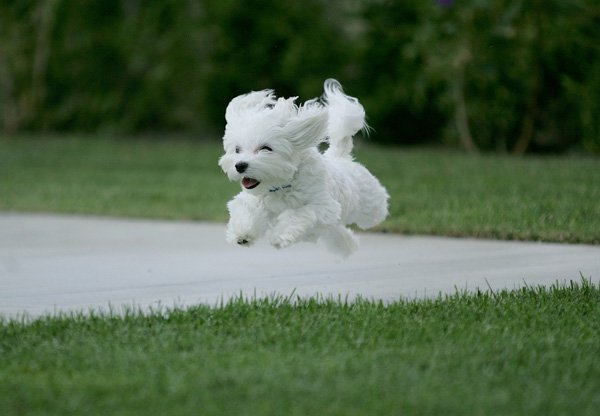
\includegraphics[width = 7.5in]{351Week7puppy2.jpg}
    \end{center}}
\end{columns}

\begin{columns}
  \column{0.5}
  \block{The Fundamental Theorem of Algebra}{\textbf{Theorem.}
    Every polynomial $f(x) = a_n x^n + \cdots + a_0$ has a root
    in $\mathbb{C}$. \\[2ex]

    \innerblock{A sktech of a proof}{

      When $r \approx 0$, we see \( f(r e^{i \theta}) \approx a_0 \).  \\[2ex]

      When $r$ is big, we see $f(r e^{i \theta}) \approx a_n r^n e^{i n \theta}$.
      These are $n$ giant circles in the complex plane.  \\[2ex]

      So as $r$ changes from $0$ to $\infty$, there are values $r, \theta$ which make
      $f(r e^{i \theta})$ cross the origin in the complex plane.}}

  \column{0.5}
  \block{An example when $f(x) = x^3 - x + 1$}{
    \begin{center}
      $f(r e^{i \theta})$ for $\theta \in [0,2 \pi)$ shown on the complex plane: \\[2ex]
      \begin{tikzpicture}[scale = 2.5]
        \node at (0,-3) {$r = .1$};
        \draw [->, thin] (-1.5,0) -- (2.5,0);
        \draw [->, thin] (0,-2) -- (0,2);
        \draw (1, .05) -- (1, -.05) node [below] {$1$};
        \draw [domain=0:2*pi, samples = 100, smooth, ultra thick, blue]
        plot ({1 - 0.1*cos(\x r) + 0.001*cos(3*\x r)},
        {-0.1*sin(\x r) + 0.001*sin(3*\x r)});
      \end{tikzpicture}
      \hspace{5ex}
      \begin{tikzpicture}[scale = 2.5]
        \node at (0,-3) {$r = .5$};
        \draw [->, thin] (-1.5,0) -- (2.5,0);
        \draw [->, thin] (0,-2) -- (0,2);
        \draw (1, .05) -- (1, -.05) node [below] {$1$};
        \draw [domain=0:2*pi, samples = 100, smooth, ultra thick, blue]
        plot ({1 - 0.5*cos(\x r) + 0.125*cos(3*\x r)},
        {-0.5*sin(\x r) + 0.125*sin(3*\x r)});
      \end{tikzpicture}
      \hspace{5ex}
      \begin{tikzpicture}[scale = 2.5]
        \node at (0,-3) {$r = .75$};
        \draw [->, thin] (-1.5,0) -- (2.5,0);
        \draw [->, thin] (0,-2) -- (0,2);
        \draw (1, .05) -- (1, -.05) node [below] {$1$};
        \draw [domain=0:2*pi, samples = 100, smooth, ultra thick, blue]
        plot ({1 - 0.75*cos(\x r) + 0.421875*cos(3*\x r)},
        {-0.75*sin(\x r) + 0.421875*sin(3*\x r)});
      \end{tikzpicture}
      \hspace{5ex}
      \begin{tikzpicture}[scale = 2.5]
        \node at (0,-3) {$r \approx 0.868837\dots$};
        \draw [->, thin] (-1.5,0) -- (2.5,0);
        \draw [->, thin] (0,-2) -- (0,2);
        \draw (1, .05) -- (1, -.05) node [below] {$1$};
        \draw [domain=0:2*pi, samples = 100, smooth, ultra thick, blue]
        plot ({1 - 0.868837*cos(\x r) + 0.655866*cos(3*\x r)},
        {-0.868837*sin(\x r) + 0.655866*sin(3*\x r)});
      \end{tikzpicture}
    \end{center}}
\end{columns}

\end{document}
